%% ============================================================
%%  Ligue 1 Match Prediction — Sam's Modeling slides (4 slides)
%%  Standalone, style-compatible with slides.tex.
%%  Frame order:
%%    1. Hyperparameters & Tuning   (random search, TimeSeriesSplit, KNN k)
%%    2. Modeling — Results          (unchanged from slides.tex)
%%    3. Modeling — Feature Importance (unchanged from slides.tex)
%%    4. Other Models                (condensed; +1 line on LR difference)
%% ============================================================
\documentclass[aspectratio=169,12pt]{beamer}

%% ── Theme ────────────────────────────────────────────────────
\usetheme{Madrid}
\setbeamertemplate{navigation symbols}{}   % remove nav icons
\setbeamertemplate{footline}{%
  \leavevmode%
  \hbox{%
    \begin{beamercolorbox}[wd=.45\paperwidth,ht=2.4ex,dp=1ex,center]{author in head/foot}%
      \usebeamerfont{author in head/foot}\insertshortauthor
    \end{beamercolorbox}%
    \begin{beamercolorbox}[wd=.45\paperwidth,ht=2.4ex,dp=1ex,center]{title in head/foot}%
      \usebeamerfont{title in head/foot}\insertshorttitle
    \end{beamercolorbox}%
    \begin{beamercolorbox}[wd=.1\paperwidth,ht=2.4ex,dp=1ex,right]{date in head/foot}%
      \insertframenumber{}/\inserttotalframenumber\hspace*{2ex}
    \end{beamercolorbox}}%
}

%% ── Colours ──────────────────────────────────────────────────
\usepackage{xcolor}
\definecolor{darkblue}{RGB}{23,55,94}
\definecolor{midblue}{RGB}{44,123,182}
\definecolor{playercol}{RGB}{231,76,60}
\definecolor{fbrefcol}{RGB}{155,89,182}
\definecolor{understcol}{RGB}{44,123,182}
\definecolor{lightgrey}{RGB}{245,245,245}

\setbeamercolor{palette primary}{bg=darkblue,fg=white}
\setbeamercolor{palette secondary}{bg=midblue,fg=white}
\setbeamercolor{palette tertiary}{bg=darkblue,fg=white}
\setbeamercolor{frametitle}{bg=darkblue,fg=white}
\setbeamercolor{title}{fg=white}
\setbeamercolor{block title}{bg=midblue,fg=white}
\setbeamercolor{block body}{bg=lightgrey,fg=black}
\setbeamercolor{alerted text}{fg=playercol}

%% ── Packages ─────────────────────────────────────────────────
\usepackage{graphicx}
\usepackage{booktabs}
\usepackage{tabularx}
\usepackage{tikz}
\usetikzlibrary{arrows.meta,shapes.geometric,positioning,calc}
\usepackage{fontawesome5}
\usepackage{array}
\usepackage{multirow}
\usepackage{amsmath}
\usepackage{eso-pic}

%% ── Circular presenter photo (top-right, page-absolute) ──────
\newcommand{\presenterphoto}[1]{%
  \AddToShipoutPictureFG*{%
    \AtPageUpperLeft{%
      \put(\LenToUnit{\paperwidth-0.62cm},\LenToUnit{-0.52cm}){%
        \tikz[overlay]{%
          \begin{scope}
            \clip (0,0) circle (0.40cm);
            \node[inner sep=0pt] at (0,0)
              {\includegraphics[width=0.82cm]{#1}};
          \end{scope}
          \draw[white,line width=0.8pt] (0,0) circle (0.40cm);
        }%
      }%
    }%
  }%
}

%% ── Metadata ─────────────────────────────────────────────────
\title[Player-Level Match Prediction]{%
  Predicting Ligue 1 Match Outcomes\\
  with Player-Level Statistics}
\subtitle{Modeling}
\author[O'Shea, Majbruch, Olaru, Sudit]{Sienna O'Shea, Samuel Majbruch, Ioana Olaru \& Ava Sudit}
\date{}

%% ═══════════════════════════════════════════════════════════
\begin{document}

\section{Modeling}

%% ═══════════════════════════════════════════════════════════
%% ── Slide 1 (Sam): Hyperparameters & Tuning ──────────────────────
%% ═══════════════════════════════════════════════════════════
\begin{frame}[t,shrink=10]{Modeling — Hyperparameters \& Tuning}
\presenterphoto{sam_ml}
  \footnotesize
  Every model is tuned with \textbf{\texttt{RandomizedSearchCV}} (random configs drawn
  from each grid below), scored by \textbf{log-loss} (\texttt{neg\_log\_loss}), not
  accuracy. Cross-validation uses \textbf{\texttt{TimeSeriesSplit} (5 folds)} so the
  validation fold is always \alert{later in time} than the training fold --- data is never
  shuffled across the time boundary. Draw imbalance is handled with \textbf{balanced class
  weights} (RF) / \textbf{sample weights} (XGB); the best estimator is then
  \textbf{isotonic-calibrated} (\texttt{CalibratedClassifierCV}, temporal inner split)
  before the 50/50 RF\,+\,XGB ensemble.

  \vspace{0.4em}
  \begin{columns}[T]
    \column{0.49\textwidth}
    \begin{block}{Random Forest — search grid}
      \scriptsize
      \setlength{\tabcolsep}{4pt}\renewcommand{\arraystretch}{1.05}
      \begin{tabular}{ll}
        \texttt{n\_estimators}     & 200 / 400 / 600 / 800 \\
        \texttt{max\_depth}        & 3 / 5 / 7 / 10 / None \\
        \texttt{min\_samples\_leaf}  & 1 / 2 / 4 / 8 \\
        \texttt{min\_samples\_split} & 2 / 5 / 10 \\
        \texttt{max\_features}     & sqrt / log2 / 0.5 \\
      \end{tabular}
    \end{block}

    \column{0.49\textwidth}
    \begin{block}{XGBoost — search grid}
      \scriptsize
      \setlength{\tabcolsep}{4pt}\renewcommand{\arraystretch}{1.05}
      \begin{tabular}{ll}
        \texttt{n\_estimators}     & 200 / 400 / 600 / 800 \\
        \texttt{max\_depth}        & 3 / 4 / 5 / 6 / 8 \\
        \texttt{learning\_rate}    & 0.01 / 0.03 / 0.05 / 0.1 \\
        \texttt{subsample}         & 0.6 / 0.8 / 1.0 \\
        \texttt{colsample\_bytree} & 0.6 / 0.8 / 1.0 \\
        \texttt{min\_child\_weight}  & 1 / 3 / 5 \quad\texttt{reg\_lambda} 0.5--5 \\
      \end{tabular}
    \end{block}
  \end{columns}

  \vspace{0.4em}
  \begin{alertblock}{\scriptsize Choosing $k$ for KNN (same protocol)}
    \scriptsize Grid $k \in \{5,10,15,20,30,50\} \times$ \{uniform, distance\} $\times$
    \{Manhattan, Euclidean\}, scored by log-loss under \texttt{TimeSeriesSplit(5)}.
    Floor $k{=}5$ (smaller gives degenerate probabilities); ceiling $k{=}50$ (smallest
    CV fold is $\sim$75 rows). All three regimes independently picked
    \textbf{$k{=}50$, distance-weighted}.
  \end{alertblock}
\end{frame}

%% ═══════════════════════════════════════════════════════════
%% ── Slide 2: Modeling Results (UNCHANGED) ──────────────────
%% ═══════════════════════════════════════════════════════════
\begin{frame}{Modeling — Results}
\presenterphoto{sam_ml}
  \begin{columns}[T]
    \column{0.58\textwidth}
    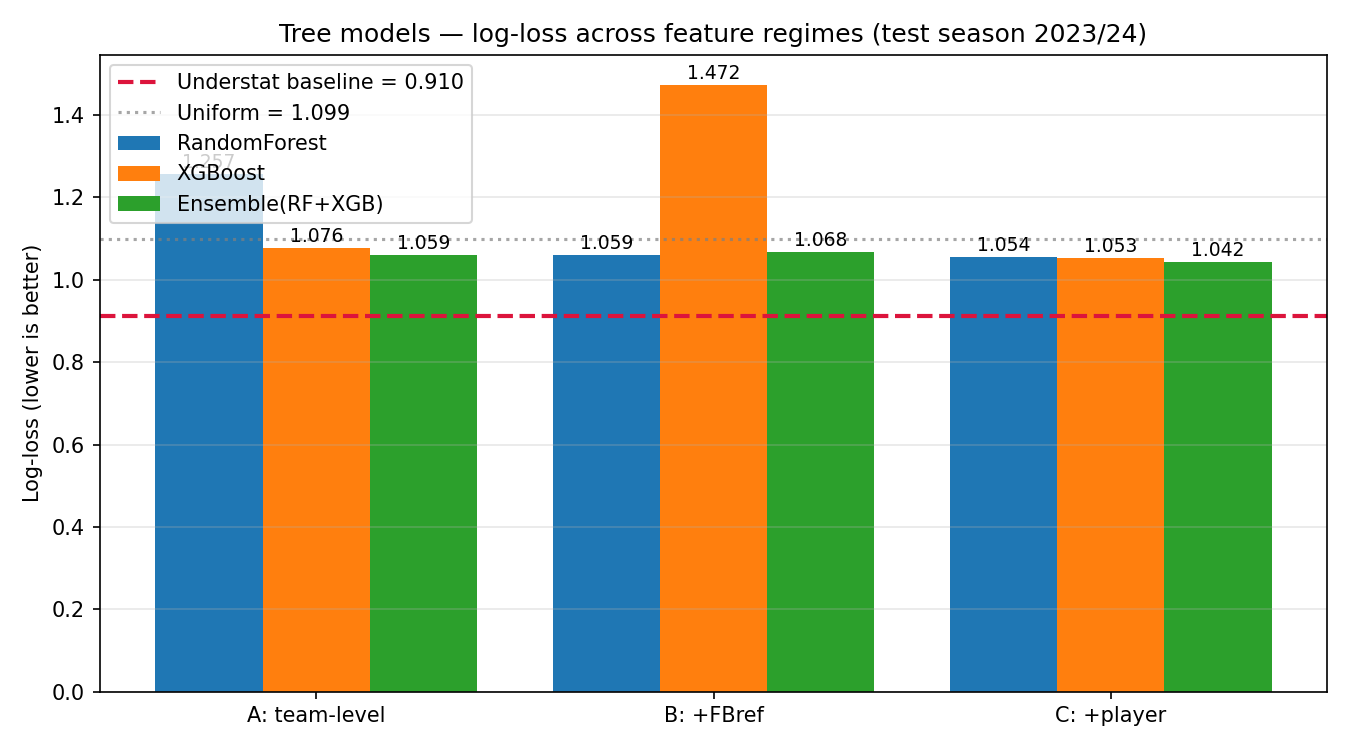
\includegraphics[width=\linewidth]{../outputs/models_tree/logloss_comparison.png}

    \column{0.40\textwidth}
    \scriptsize\textbf{Test log-loss (season 2023/24)}\\[0.3em]
    \setlength{\tabcolsep}{4pt}
    \begin{tabular}{lccc}
      & \textbf{A} & \textbf{B} & \textbf{C} \\
      \hline
      RF                & 1.26 & 1.06 & 1.05 \\
      XGB               & 1.08 & 1.47 & 1.05 \\
      \textbf{Ensemble} & 1.06 & 1.07 & \alert{\textbf{1.04}} \\
      \hline
      LR (ref)          & 1.06 & 1.14 & 1.22 \\
    \end{tabular}\\[0.2em]
    \textit{\textbf{A}=team, \textbf{B}=+FBref, \textbf{C}=+player}

    \vspace{0.4em}
    \textbf{Accuracy in context (3-class):}\\[0.2em]
    \setlength{\tabcolsep}{3pt}
    \begin{tabular}{lc}
      Random guess & 33\% \\
      Always home  & 43\% \\
      Best model   & 50\% \\
      Bookmaker    & \textbf{56\%} \\
    \end{tabular}

    \vspace{0.4em}
    \alert{\textbf{No model clears the bookmaker baseline
    (0.91 log-loss).}} Bookmakers have real-time info
    (injuries, team news) that rolling historical stats
    cannot capture.
  \end{columns}
\end{frame}

%% ═══════════════════════════════════════════════════════════
%% ── Slide 3: Feature Importance (UNCHANGED) ────────────────
%% ═══════════════════════════════════════════════════════════
\begin{frame}{Modeling — Feature Importance (XGBoost, full regime)}
\presenterphoto{sam_ml}
  \begin{columns}[T]
    \column{0.58\textwidth}
    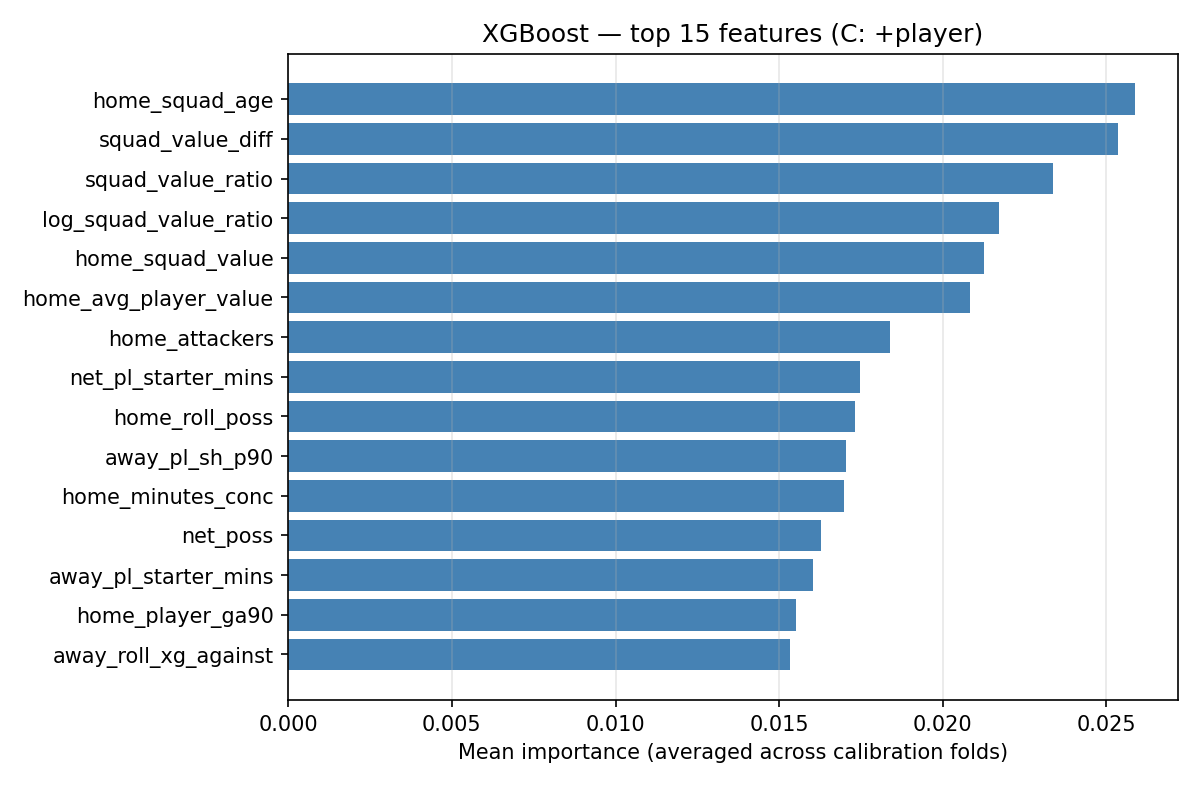
\includegraphics[width=\linewidth]{../outputs/models_tree/importance_c_player_xgboost.png}

    \column{0.40\textwidth}
    \footnotesize\textbf{How to read:} mean importance over the calibration
    folds for the best XGBoost on the full player regime.

    \vspace{0.6em}
    \textbf{Team-level form} (rolling xG, market value) sits at the top,
    as expected.

    \vspace{0.6em}
    \textcolor{playercol}{\textbf{Player-level features}}
    (\texttt{starter\_mins}, \texttt{pct\_fw}, depth gaps) appear
    repeatedly in the top ranks — they are not just noise the model
    tolerates, they are signal the model actively uses.

    \vspace{0.6em}
    Consistent with the feature-selection leaderboard
    (\texttt{net\_pl\_starter\_mins} rank~9, \texttt{net\_pl\_pct\_fw} rank~11).
  \end{columns}
\end{frame}

%% ═══════════════════════════════════════════════════════════
%% ── Slide 4: Other Models ──────────────────────────────────
%% ═══════════════════════════════════════════════════════════
\begin{frame}[t,shrink=6]{Modeling — Other Models}
\presenterphoto{sam_ml}
  \footnotesize Same protocol, same temporal holdout, same 3 regimes — four more
  model families, to test whether the algorithm matters at our sample size.

  \vspace{0.3em}
  \begin{columns}[T]
    \column{0.55\textwidth}
    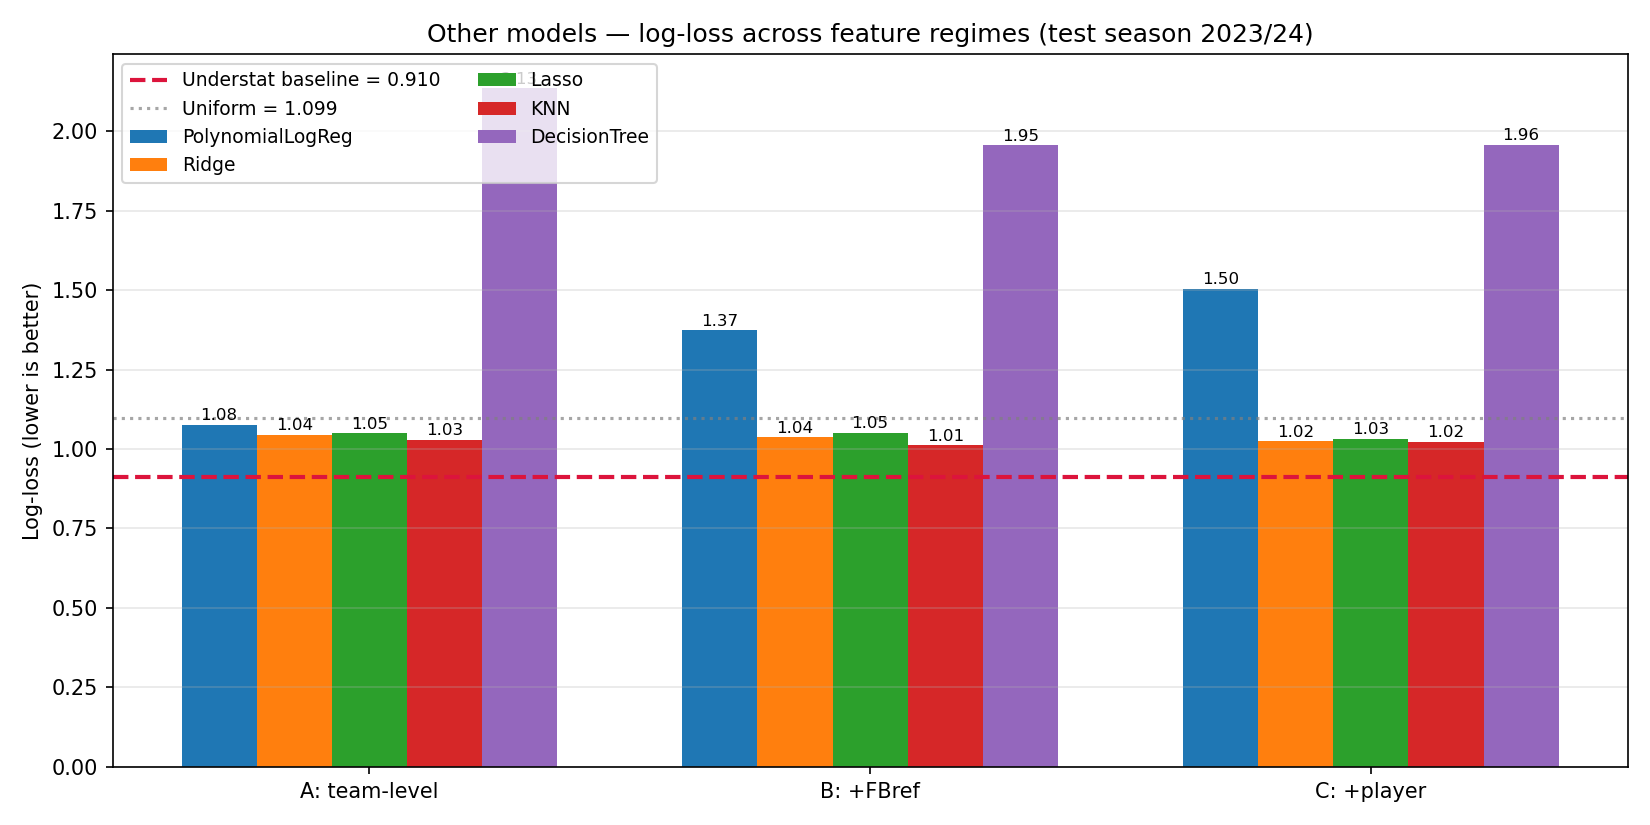
\includegraphics[width=\linewidth]{../outputs/other_models/logloss_comparison.png}

    \column{0.42\textwidth}
    \scriptsize\textbf{Test log-loss (season 2023/24)}\\[0.2em]
    \setlength{\tabcolsep}{3pt}
    \begin{tabular}{lccc}
      & \textbf{A} & \textbf{B} & \textbf{C} \\
      \hline
      Polynomial    & 1.08 & 1.37 & 1.50 \\
      Ridge (L2)    & 1.04 & 1.04 & \textbf{1.02} \\
      Lasso (L1)    & 1.05 & 1.05 & 1.03 \\
      KNN           & 1.03 & \alert{\textbf{1.01}} & 1.02 \\
      Decision Tree & 2.13 & 1.96 & 1.96 \\
      \hline
      RF+XGB ens.   & 1.06 & 1.07 & 1.04 \\
    \end{tabular}\\[0.4em]
    \textit{\textbf{A}=team, \textbf{B}=+FBref, \textbf{C}=+player}

    \vspace{0.4em}
    \alert{\textbf{Six algorithms cluster within 0.03 log-loss}}
    — we've hit the \emph{information ceiling} of post-match aggregate
    stats. Closing the gap to Understat (0.91) needs richer features,
    not a different model.
  \end{columns}

  \vspace{0.3em}
  \footnotesize\textbf{Per-model takeaways:}
  \textbf{Polynomial} overfits as features grow ($d{=}2$ explodes to $400^+$ inputs);
  \textbf{Ridge/Lasso} match each other — regularisation type barely matters here;
  \textbf{KNN} ties the tree ensemble (small dataset $\to$ simple wins);
  \textbf{Decision Tree} is worst in every regime — confirming the value of bagging/boosting.

  \vspace{0.2em}
  \footnotesize\textit{\textbf{Why this differs from Logistic Regression:} LR \emph{worsened}
  as features were added (1.06 $\to$ 1.14 $\to$ 1.22) under multicollinearity and the
  curse of dimensionality; trees and regularised / instance-based models instead hold or
  \alert{improve} with the extra player features — they handle correlated inputs natively.}
\end{frame}

\end{document}
